\chapter{Solución Propuesta}

\section{Propuesta de Solución}
Se elaboró un sistema de realidad virtual del sistema digestivo del cuerpo humano que permite interactuar con modelos tridimensionales. La intención es sentar las bases
 para un sistema de apoyo al aprendizaje que sea más práctico \cite{moore1995learning}, sin sustituir a ningún método de estudio tradicional.\\

\section{Viabilidad} \label{viab}
También se analizó la factibilidad del proyecto en general. Desde el punto de vista técnico se realizó una evaluación de la tecnología actual existente y la posibilidad de 
utilizarla en el desarrollo del sistema. Además de DirectX versión 11 el cuadro \ref{tab:t23} muestra los recursos técnicos necesarios para la ejecución correcta del software:\\
\begin{table}[H]
\centering
\begin{tabular}{|c|c|l|}
\hline
\rowcolor[HTML]{9B9B9B} 
\textbf{Cantidad} &
  \textbf{Recursos} &
  \multicolumn{1}{c|}{\cellcolor[HTML]{9B9B9B}\textbf{Características}} \\ \hline
\cellcolor[HTML]{C0C0C0}1 &
  Computadora Personal de Escritorio &
  \begin{tabular}[c]{@{}l@{}}Tarjeta gráfica discreta, RX480\\ Memoria RAM 16 Gb\\ 5 Puertos USB\\ Procesador de 4 núcleos o mayor\end{tabular} \\ \hline
\cellcolor[HTML]{C0C0C0}1 &
  Sistema de realidad Virtual Oculus Rift &
  \begin{tabular}[c]{@{}l@{}}Visor HMD, controles Touch \\ \\ Sensores Touch.\end{tabular} \\ \hline
\end{tabular}
\caption{ Recursos Técnicos.}
\label{tab:t23}
\end{table}
Económicamente, se determinaron los recursos para desarrollar el sistema así como la comparativa con el uso de cuerpos para su examinación y estudio. Después de un análisis e 
investigación de los costos con la dirección del Área de Morfología en la Escuela Superior de Medicina bajo la asesoría del Dr. Macias Rios se determinó que el costo que se 
tiene para el traslado, mantenimiento, uso e inhumación de los cuerpos es de \$40,000.00 c/u, como se ve en el cuadro \ref{tab:t24}.
\begin{table}[H]
\centering
\begin{tabular}{|
>{\columncolor[HTML]{C0C0C0}}c |l|}
\hline
\multicolumn{2}{|c|}{\cellcolor[HTML]{9B9B9B}\textbf{Costo de uso de cuerpos.}} \\ \hline
Traslado, mantenimiento, uso e inhumación           & \$40,000.00 c/u           \\ \hline
Total                                               & \$40,000.00 c/u           \\ \hline
\end{tabular}
\caption{Costo de cálculo de uso de cuerpos.}
\label{tab:t24}
\end{table}

En el caso del desarrollo e implementación del proyecto se consideró la depreciación, como se observa en el cuadro \ref{tab:t25}.
\begin{table}[H]
\centering
\resizebox{\textwidth}{!}{%
\begin{tabular}{clccccc|c|c|}
\hline
\rowcolor[HTML]{9B9B9B} 
\multicolumn{9}{|c|}{\cellcolor[HTML]{9B9B9B}\textbf{Depreciaciones del Proyecto}} \\ \hline
\rowcolor[HTML]{9B9B9B} 
\multicolumn{4}{|c|}{\cellcolor[HTML]{9B9B9B}\textbf{Equipos de Cómputo}} &
  \multicolumn{5}{c|}{\cellcolor[HTML]{9B9B9B}\textbf{Depreciación}} \\ \hline
\rowcolor[HTML]{9B9B9B} 
\multicolumn{1}{|c|}{\cellcolor[HTML]{9B9B9B}\textbf{Cantidad}} &
  \multicolumn{1}{c|}{\cellcolor[HTML]{9B9B9B}\textbf{Equipos}} &
  \multicolumn{1}{c|}{\cellcolor[HTML]{9B9B9B}\textbf{\begin{tabular}[c]{@{}c@{}}Monto original de \\ Inversión\end{tabular}}} &
  \multicolumn{1}{c|}{\cellcolor[HTML]{9B9B9B}\textbf{\begin{tabular}[c]{@{}c@{}}Valor actual\\  del equipo\end{tabular}}} &
  \multicolumn{1}{c|}{\cellcolor[HTML]{9B9B9B}\textbf{\begin{tabular}[c]{@{}c@{}}Valor a \\ \\ depreciar\end{tabular}}} &
  \multicolumn{1}{c|}{\cellcolor[HTML]{9B9B9B}\textbf{\begin{tabular}[c]{@{}c@{}}\%\\ anual\end{tabular}}} &
  \textbf{\begin{tabular}[c]{@{}c@{}}\%\\ mensual\end{tabular}} &
  \textbf{\begin{tabular}[c]{@{}c@{}}Depresiación\\ mensual\end{tabular}} &
  \textbf{\begin{tabular}[c]{@{}c@{}}Depreciación\\ anual\end{tabular}} \\ \hline
\multicolumn{1}{|c|}{\cellcolor[HTML]{C0C0C0}1} &
  \multicolumn{1}{l|}{\begin{tabular}[c]{@{}l@{}}Computadora de\\ escritorio armada\end{tabular}} &
  \multicolumn{1}{c|}{\$25,054.63} &
  \multicolumn{1}{c|}{\$20,000.00} &
  \multicolumn{1}{c|}{\$5,054.63} &
  \multicolumn{1}{c|}{33.33\%} &
  2.78\% &
  \$ 140.52 &
  \$1,545.72 \\ \hline
\multicolumn{1}{|c|}{\cellcolor[HTML]{C0C0C0}1} &
  \multicolumn{1}{l|}{Laptop HP} &
  \multicolumn{1}{c|}{\$9,999.00} &
  \multicolumn{1}{c|}{\$6,999.00} &
  \multicolumn{1}{c|}{\$3,000.00} &
  \multicolumn{1}{c|}{33.33\%} &
  2.78\% &
  \$ 83.40 &
  \$ 917.40 \\ \hline
\multicolumn{7}{l}{} &
  \textbf{Total:} &
  \$ 2,463.12 \\ \cline{8-9} 
\end{tabular}
}
\caption{Depreciaciones del proyecto.}
\label{tab:t25}
\end{table}

Para ofrecer una experiencia aceptable al momento del uso del equipo de Realidad Virtual y el software se proponen los elementos del cuadro \ref{tab:t26}.
%%
  %Tabla de costos de productos, no se ha logrado realizar correctamente%
%%
\textbf{Pendiente tabla costos}\\
Además, el sistema de Realidad Virtual con sus componentes tiene un costo que se muestra en el cuadro \ref{tab:t27}.
\begin{table}[H]
  \centering
  \begin{tabular}{|c|c|}
  \hline
  \rowcolor[HTML]{9B9B9B} 
  \multicolumn{2}{|c|}{\cellcolor[HTML]{9B9B9B}\textbf{Sistema de Realidad Virtual}} \\ \hline
  \rowcolor[HTML]{9B9B9B} 
  \textbf{Producto}                          & \textbf{Producto}                     \\ \hline
  Visor Oculus Rift                          & Incluido en el paquete                \\ \hline
  Controles Touch Oculus x 2                 & Incluido en el paquete                \\ \hline
  Sensores Oculus x 2                        & Incluido en el paquete                \\ \hline
  Anexos                                     & Incluido en el paquete                \\ \hline
  \textbf{Total:}                            & \$ 8,821.74                           \\ \hline
  \end{tabular}
  \caption{Costos y contenido del sistema de Realidad Virtual.}
  \label{tab:t27}
\end{table}

Se estimaron los sueldos de programador y modelado, como se observa en el cuadro \ref{tab:t28}.\\
\begin{table}[H]
  \centering
  \resizebox{\textwidth}{!}{%
  \begin{tabular}{ccc|c|c|}
  \hline
  \rowcolor[HTML]{9B9B9B} 
  \multicolumn{5}{|c|}{\cellcolor[HTML]{9B9B9B}\textbf{Sueldos}}                                                                                                                                                                                                                                                                    \\ \hline
  \rowcolor[HTML]{9B9B9B} 
  \multicolumn{1}{|c|}{\cellcolor[HTML]{9B9B9B}\textbf{Puesto}} & \multicolumn{1}{c|}{\cellcolor[HTML]{9B9B9B}\textbf{\begin{tabular}[c]{@{}c@{}}Sueldo\\ Mensual\\ individual\end{tabular}}} & \textbf{\begin{tabular}[c]{@{}c@{}}Cantidad \\ \\ de personal\end{tabular}} & \textbf{Sueldos mensuales totales} & \textbf{6 meses} \\ \hline
  \multicolumn{1}{|c|}{Programador}                             & \multicolumn{1}{c|}{\$25,296.00}                                                                                            & 1                                                                           & \$25,296.00                        & \$151,776.00     \\ \hline
  \multicolumn{1}{|c|}{Modelador 3D}                            & \multicolumn{1}{c|}{\$25,296.00}                                                                                            & 1                                                                           & \$25,296.00                        & \$151,776.00     \\ \hline
  \multicolumn{3}{l}{}                                                                                                                                                                                                                                                      & \multicolumn{1}{l|}{Total}         & \$303,522.00     \\ \cline{4-5} 
  \end{tabular}%
  }
  \caption{Cálculo de Sueldos.
  }
  \label{tab:t28}
\end{table}

\begin{table}[H]
  \centering
  \begin{tabular}{c|c|c|}
  \hline
  \rowcolor[HTML]{9B9B9B} 
  \multicolumn{3}{|c|}{\cellcolor[HTML]{9B9B9B}\textbf{Servicios}}                                       \\ \hline
  \rowcolor[HTML]{9B9B9B} 
  \multicolumn{1}{|c|}{\cellcolor[HTML]{9B9B9B}\textbf{Concepto}} & \textbf{Mensual} & \textbf{11 Meses} \\ \hline
  \multicolumn{1}{|c|}{Luz (kw Consumidos por costo Unitario)}    & \$430            & \$4,730           \\ \hline
  \multicolumn{1}{|c|}{Agua (Lt consumidos por costo unitario)}   & \$200            & \$2,200           \\ \hline
  \multicolumn{1}{|c|}{Teléfono e Internet (renta mensual fija)}  & \$ 450           & \$4,850           \\ \hline
  \multicolumn{1}{l|}{}                                           & Total:           & \$11,780          \\ \cline{2-3} 
  \end{tabular}
  
  \caption{Cálculo de Costo por Servicios.}
  \label{tab:t29}
\end{table}

Los servicios estimados se muestran en el cuadro \ref{tab:t29} y en el cuadro \ref{tab:t210} se muestra la suma total y como resultado se obtiene el costo total del proyecto, 
que se estima en: \$326,316.86.\\
\begin{table}[H]
  \centering
  \begin{tabular}{|l|r|}
  \hline
  \rowcolor[HTML]{9B9B9B} 
  \multicolumn{2}{|c|}{\cellcolor[HTML]{9B9B9B}\textbf{Costos del Proyecto}}                                                    \\ \hline
  \rowcolor[HTML]{9B9B9B} 
  \multicolumn{1}{|c|}{\cellcolor[HTML]{9B9B9B}\textbf{Concepto}} & \multicolumn{1}{c|}{\cellcolor[HTML]{9B9B9B}\textbf{Costo}} \\ \hline
  Servicios                                                       & \$ 11,780                                                   \\ \hline
  Sueldos                                                         & \$303,522.00                                                \\ \hline
  Depreciaciones                                                  & \$2,463.12                                                  \\ \hline
  Equipo extra.                                                   & \$ 8,821.74                                                 \\ \hline
  Total                                                           & \$ 326,316.86                                               \\ \hline
  \end{tabular}
  \caption{Costos finales del proyecto}
  \label{tab:t210}
  \end{table}

En resumen, el costo de usar nueve cuerpos sería de \$360,000.00 y el del proyecto de \$326,318.00, con lo cual se puede considerar viable económicamente.\\

\section{Metodología}

\subsection{OpenUP}

\subsection{Metodología de Ingeniería de Software Multimedia}

\subsection{Complicaciones del desarrollo sin metodología}
El proyecto comenzó su desarrollo sin tomar en cuenta la metodología de desarrollo Open UP, lo cual detonó en que el trabajo se viera mermado en cuanto a su documentación y desarrollo.\\
El desarrollo de un sistema mediante Open UP puede ser una herramienta poderosa para el desarrollo de software ya que dentro de ella se desarrollan micro incrementos en el desarrollo del software y además cumple con los principios del Manifiesto Ágil\cite{beck2001manifesto}.\\
La problemática surge cuando se intenta implementar en un proyecto de software diferente al cual usualmente se desarrolla, por ejemplo un Sistema de Calendarización de Trabajos terminales o un Generador de Páginas Web, difiere en cuanto a su desarrollo ya que se usan herramientas y elementos diferentes, tales como el desarrollo en el motor Unity ®, el diseño de los modelos 3D y el uso de elementos propietarios de Oculus ® dificultan la tarea de documentación y desarrollo bajo lineamientos por más ligeros que sean debido a la naturaleza del proyecto.\\
Es por eso que se buscó como alternativa una metodología que tome en cuenta las características inherentes de un software que su núcleo está arraigado a la realidad virtual haciéndolo un software multimedia.\\
Debido al cambio de enfoque de desarrollo de la metodología las tareas de reingeniería son suplementadas por más tiempo de desarrollo y refinamiento de los elementos anteriores a estos dentro del cronograma de actividades.\\

\section{Modelos 3D de los Organos}
Los componentes multimedia a desarrollar en modelos 3D los cuales son miembros del sistema digestivo del ser humano, 
el sistema digestivo incluye a los órganos del tubo alimenticio y glándulas de secreción exocrina y endocrina.\\

\subsection{Glándulas Salivales}
 continuación se muestran las figuras del resultado final del desarrollo de las glándulas salivales del sistema digestivo 
 en el software de modelado en 3D llamado “Blender”, este fue realizado basado en el material anteriormente provisto.\\
\begin{figure}[H]
	\begin{center}
 		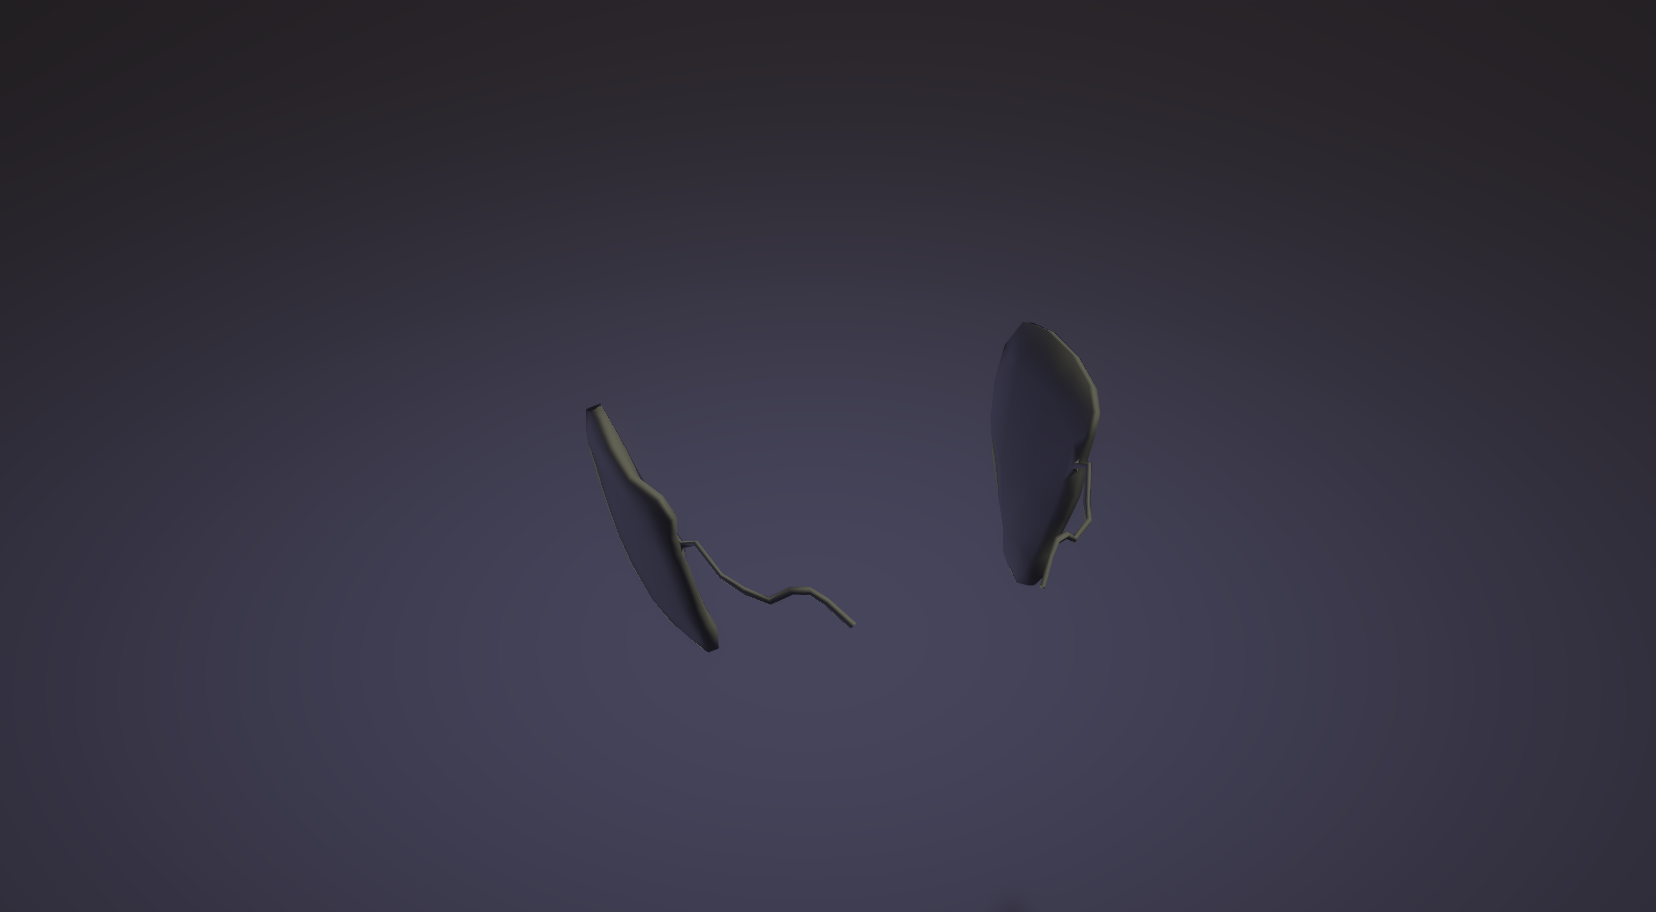
\includegraphics[width = .5\textwidth]{source/images/image41.png}
 		\captionof{figure}{\label{fig:im34}Modelo 3D de las glándulas salivales}
	\end{center} 
\end{figure}

\subsection{Cavidad oral y faringe}
A continuación se muestran las figuras del resultado final del desarrollo de la cavidad oral del sistema digestivo en el software de modelado en 3D llamado “Blender”, este fue realizado basado en el material anteriormente provisto.\\
\begin{figure}[H]
	\begin{center}
 		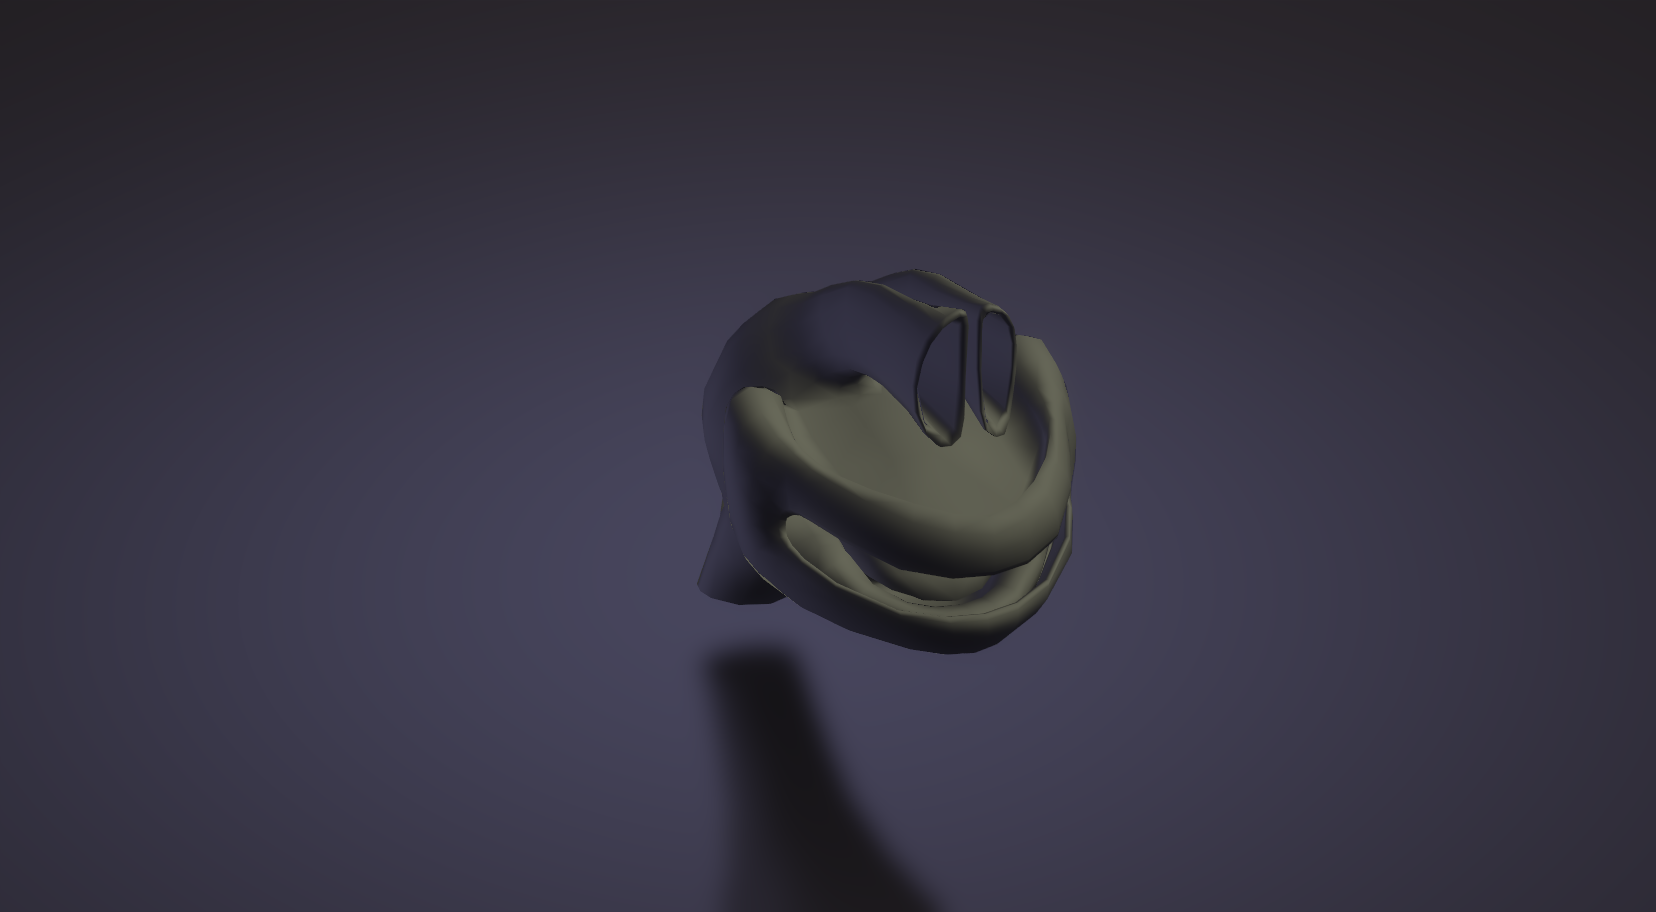
\includegraphics[width = .5\textwidth]{source/images/image14.png}
 		\captionof{figure}{\label{fig:im35}Modelo 3D de la cavidad oral}
	\end{center} 
\end{figure}

\subsection{Esófago}
A continuación se muestran las figuras del resultado final del desarrollo del esófago del sistema digestivo en el software de modelado en 3D llamado “Blender”, este fue realizado basado en el material anteriormente provisto.\\
\begin{figure}[H]
	\begin{center}
 		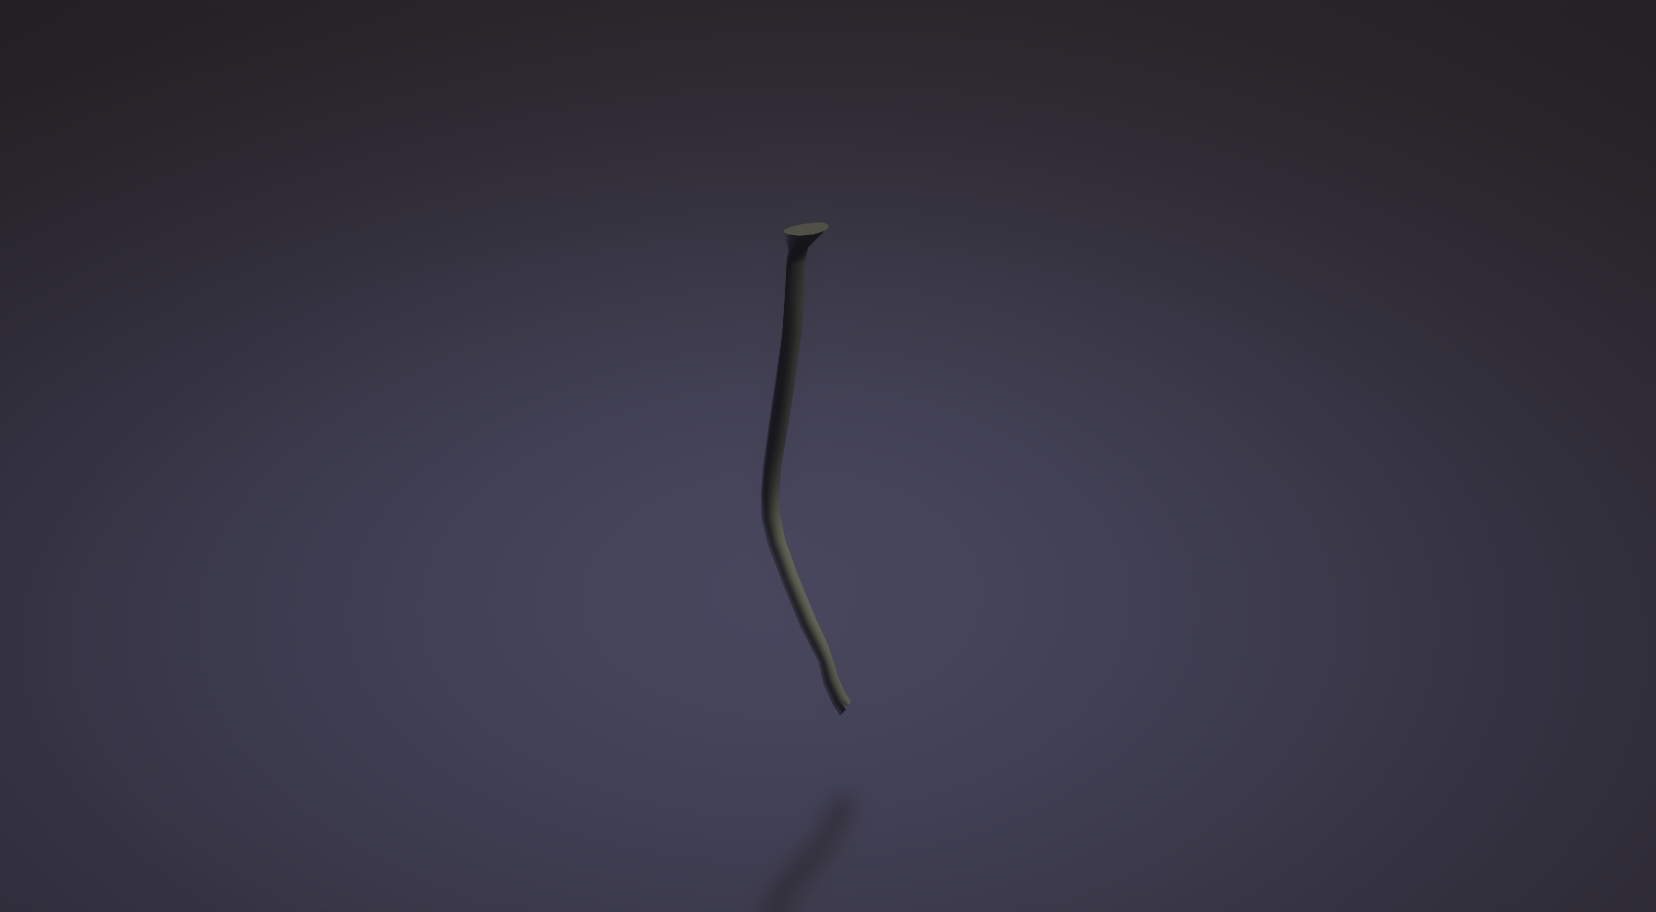
\includegraphics[width = .5\textwidth]{source/images/image25.png}
 		\captionof{figure}{\label{fig:im36}Modelo 3D del esófago}
	\end{center} 
\end{figure}

\subsection{Estómago}
A continuación se muestran las figuras del resultado final del desarrollo del estómago del sistema digestivo en el software de modelado en 3D llamado “Blender”, este fue realizado basado en el material anteriormente provisto.\\
\begin{figure}[H]
	\begin{center}
 		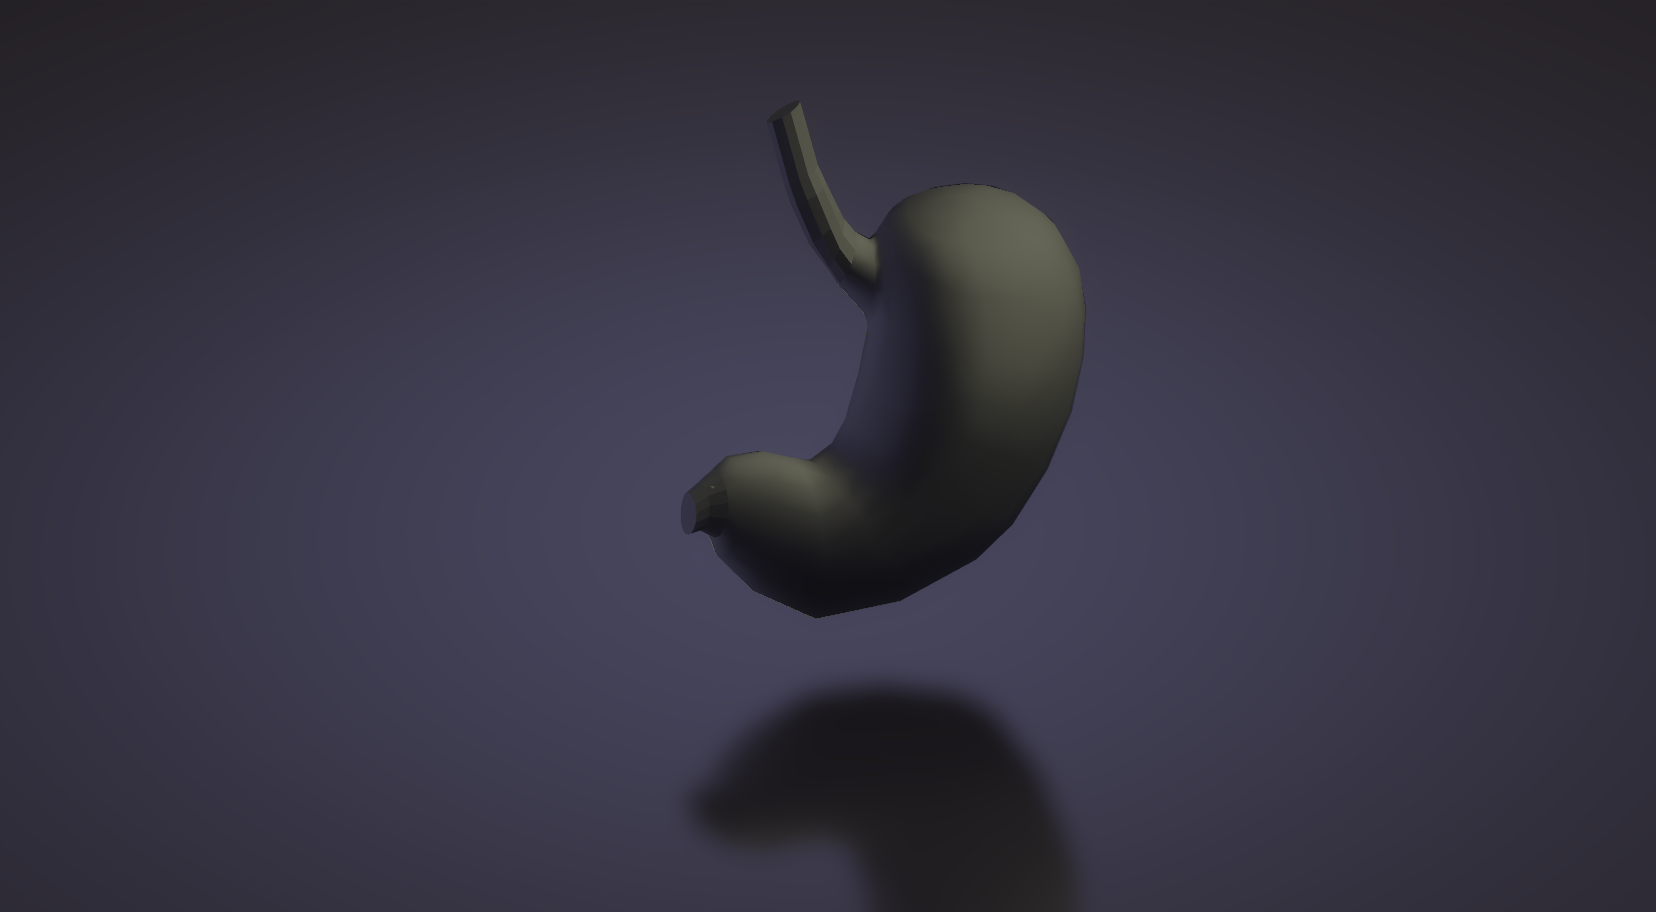
\includegraphics[width = .5\textwidth]{source/images/image42.png}
 		\captionof{figure}{\label{fig:im37} Modelo 3D del estómago }
	\end{center} 
\end{figure}

\subsection{Intestino delgado}
A continuación se muestran las figuras del resultado final del desarrollo del intestino delgado del sistema digestivo en el software de modelado en 3D llamado “Blender”, este fue realizado basado en el material anteriormente provisto.\\
\begin{figure}[H]
	\begin{center}
 		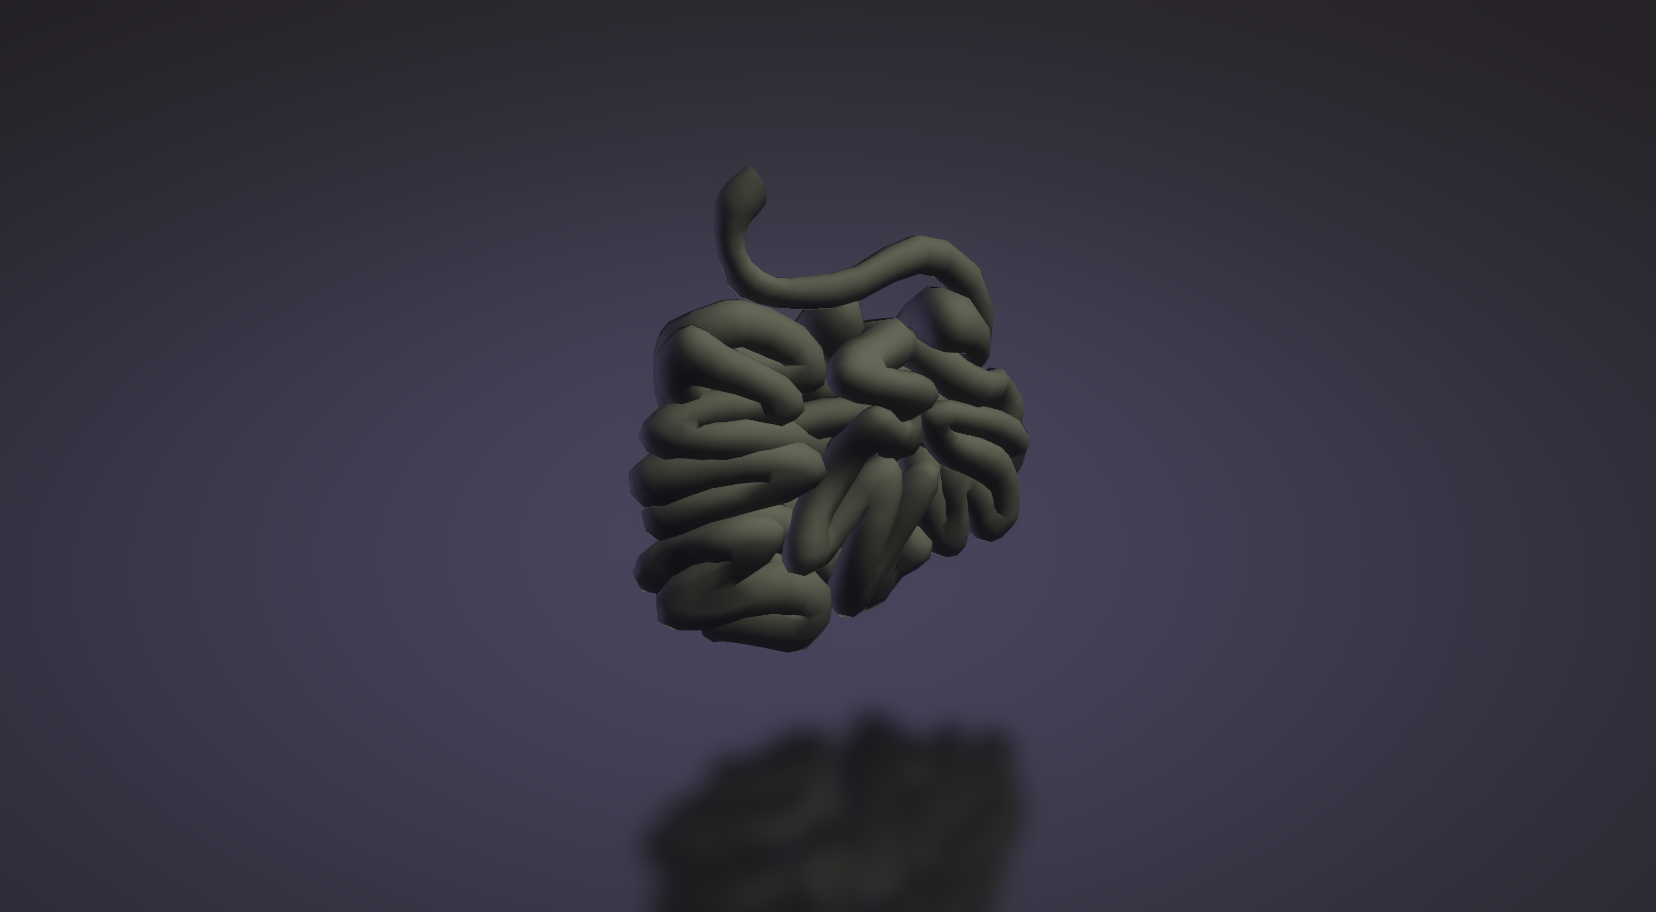
\includegraphics[width = .5\textwidth]{source/images/image69.png}
 		\captionof{figure}{\label{fig:im38}Modelo 3D del intestino delgado}
	\end{center} 
\end{figure}

\subsection{Hígado}
A continuación se muestran las figuras del resultado final del desarrollo del hígado del sistema digestivo en el software de modelado en 3D llamado “Blender”, este fue realizado basado en el material anteriormente provisto.\\
\begin{figure}[H]
	\begin{center}
 		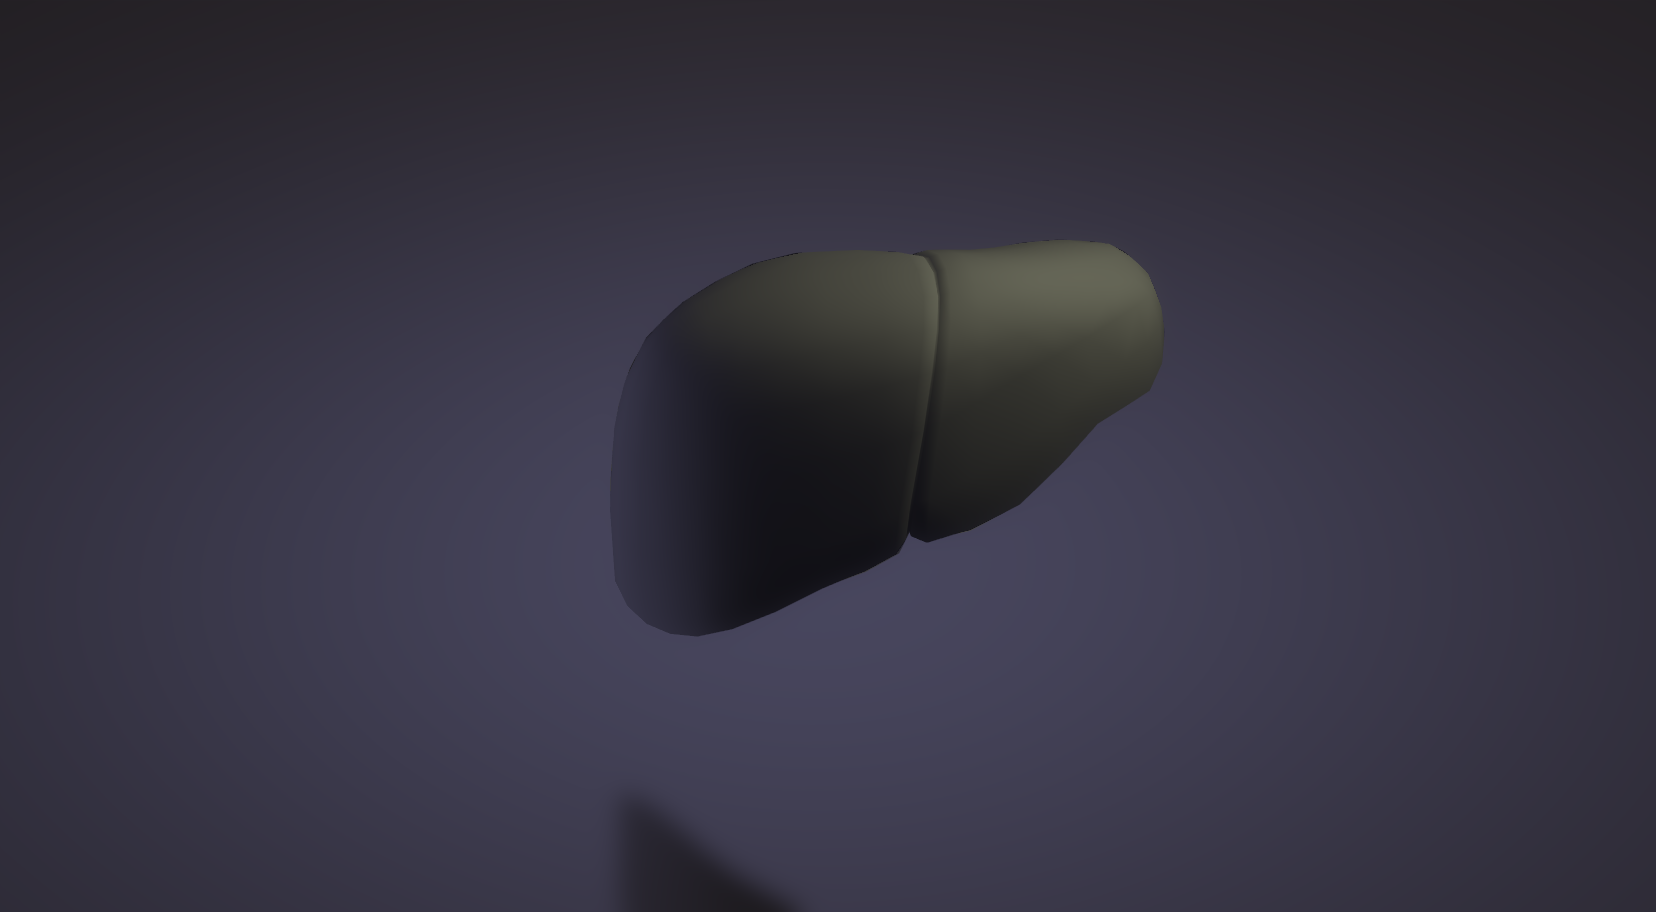
\includegraphics[width = .5\textwidth]{source/images/image17.png}
 		\captionof{figure}{\label{fig:im39}Modelo 3D del hígado}
	\end{center} 
\end{figure}

\subsection{Páncreas}
A continuación se muestran las figuras del resultado final del desarrollo del páncreas del sistema digestivo en el software de modelado en 3D llamado “Blender”, este fue realizado basado en el material anteriormente provisto.\\
\begin{figure}[H]
	\begin{center}
 		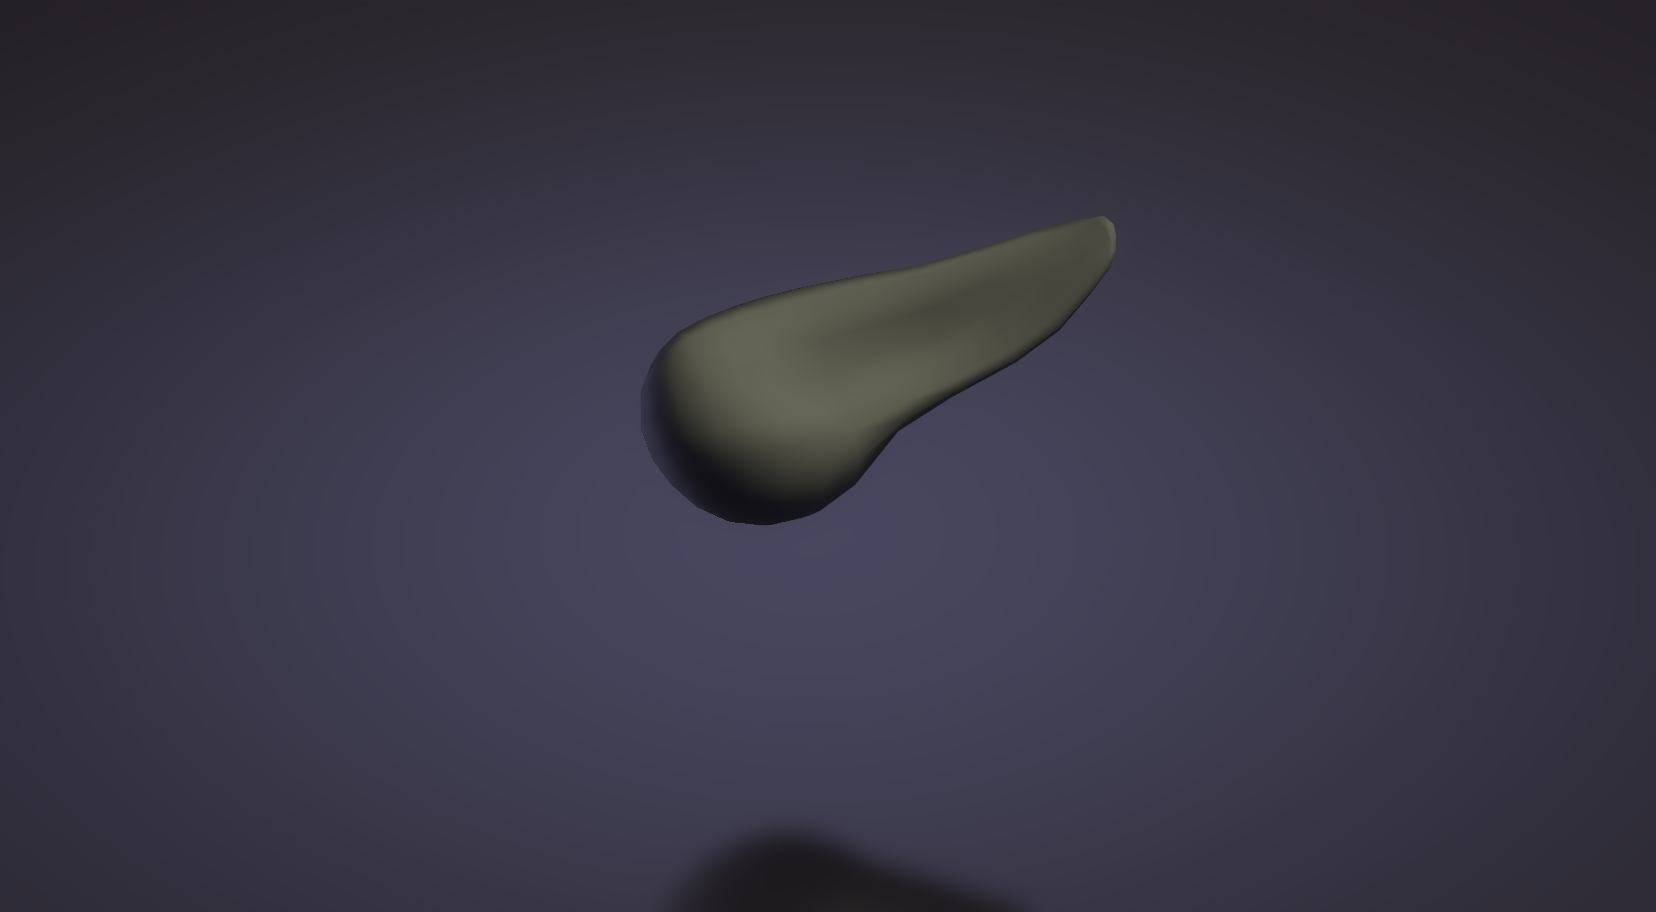
\includegraphics[width = .5\textwidth]{source/images/image19.png}
 		\captionof{figure}{\label{fig:im310}Modelo 3D del páncreas}
	\end{center} 
\end{figure}

\subsection{Vesícula Biliar}
A continuación se muestran las figuras del resultado final del desarrollo de la vesícula biliar del sistema digestivo en el software de modelado en 3D llamado “Blender”, este fue realizado basado en el material anteriormente provisto.\\
\begin{figure}[H]
	\begin{center}
 		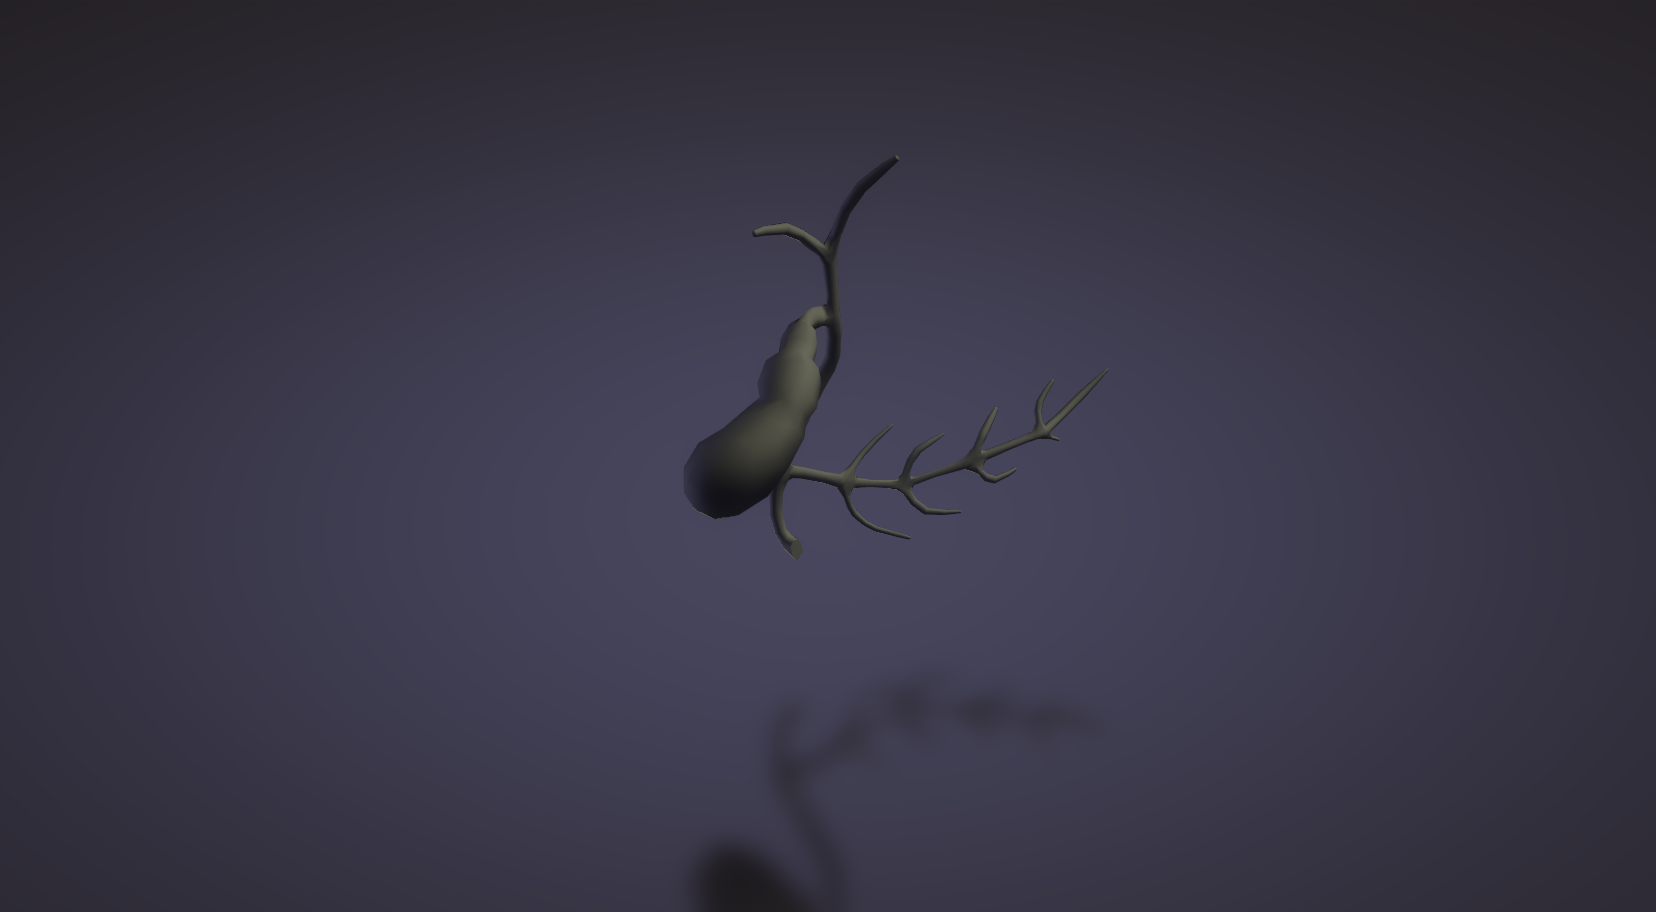
\includegraphics[width = .5\textwidth]{source/images/image26.png}
 		\captionof{figure}{\label{fig:im312}Modelo 3D de la vesícula biliar}
	\end{center} 
\end{figure}

\subsection{Intestino Grueso y Ano}
A continuación se muestran las figuras del resultado final del desarrollo del intestino grueso y ano del sistema digestivo en el software de modelado en 3D llamado “Blender”, este fue realizado basado en el material anteriormente provisto.\\
\begin{figure}[H]
	\begin{center}
 		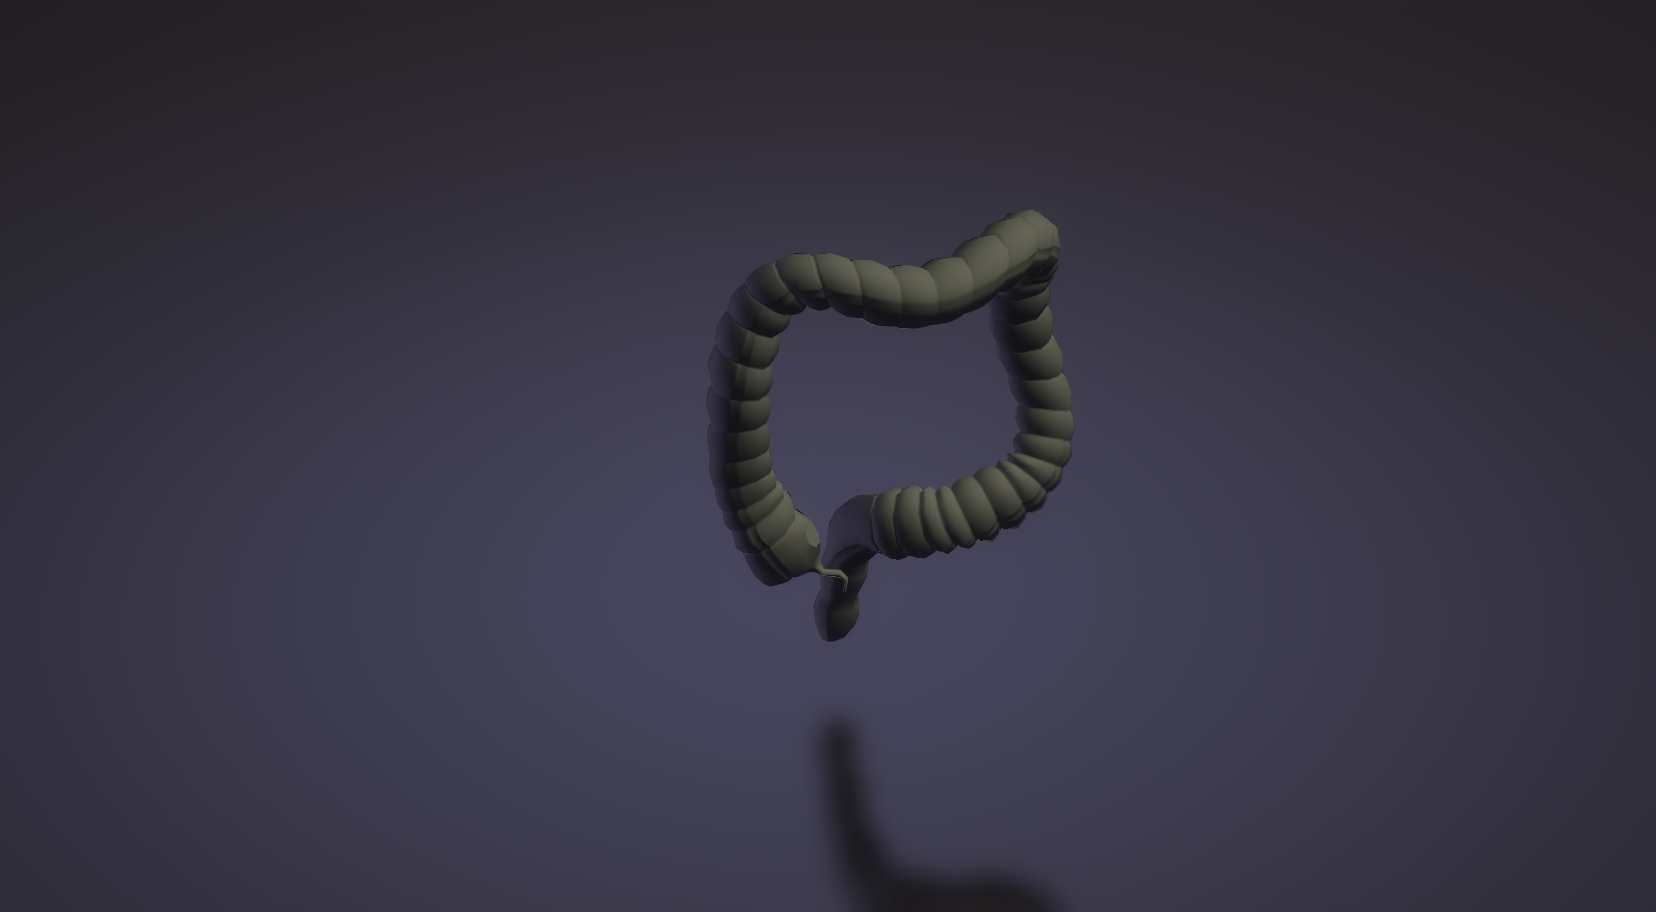
\includegraphics[width = .5\textwidth]{source/images/image20.png}
 		\captionof{figure}{\label{fig:im313}Modelo 3D del intestino grueso}
	\end{center} 
\end{figure}

\section{Modelo del sistema digestivo unificado}
A continuación se muestran las figuras del resultado final del desarrollo del sistema digestivo en el software de modelado en 3D llamado “Blender”, este fue realizado reuniendo todos los modelos de órganos y elementos individuales creados con anterioridad.\\
\begin{figure}[H]
	\begin{center}
 		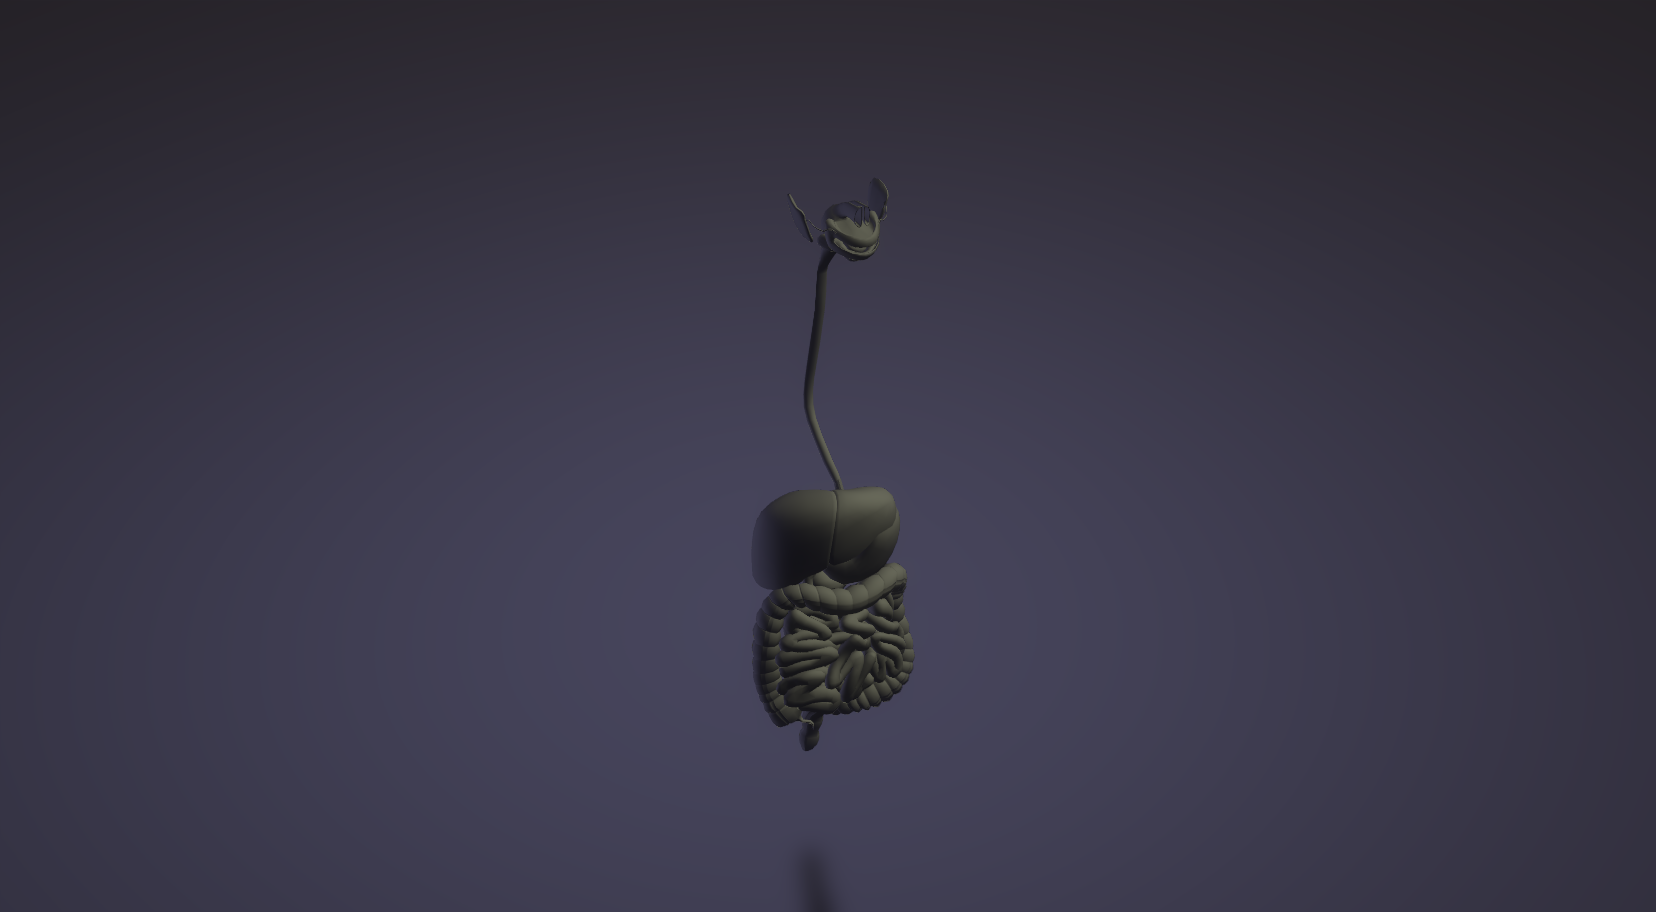
\includegraphics[width = 1\textwidth]{source/images/image24.png}
 		\captionof{figure}{\label{fig:im314}Modelo 3D del Sistema digestivo}
	\end{center} 
\end{figure}

\section{Evaluación de modelos 3D por personal calificado}
Debido al tiempo de desarrollo, el cual tomó más de lo planteado, de los modelos antes expuestos en la sección anterior no fue posible concretar una cita 
para su evaluación con el personal calificado  de la Escuela Superior de Medicina en las fechas previamente planteadas.\\
Se esperaba poder tener una reunión en fechas posteriores pero la situación epidémica que se ha desarrollado en el país y 
limitaciones impuestas por las autoridades hicieron imposible la evaluación de los modelos desarrollados.\\
Esto no significa que no se haya hecho bajo rigor alguno, sólo se utilizaron materiales de medicina impresos, así como 
referencias en video de disecciones del sistema digestivo, esto para estar lo más familiarizado posible, como estudiante 
de ingeniería en sistemas computacionales, al momento de desarrollar dichos modelos.\\
